\section{Residual Weighting}\label{sec:resWeight}

As discussed in the derivations of PROMs in Sections~\ref{sec:classicROMs} and~\ref{sec:mplsvt}, practical engineering systems are often described by state variables of vastly different magnitudes. In the case of fluid flows in rocket combustors, density (and transported scalars) are usually $\bigO{1\text{-}10}$ kg/m$^3$, velocity (and momentum) are usually $\bigO{100}$ m/s (kg/m$^2$-s), temperatures are often $\bigO{1,000}$ K, and pressures are in excess of $\bigO{1\times10^6}$ Pa. As a result, it is often important to non-dimensionalize or precondition these systems to ensure proper linear solver convergence, as the dimensional system may be poorly conditioned.

A similar notion is relevant to LSPG and MP-LSVT PROMs, whose un-normalized formulation is given respectively by
%
\begin{align}
    \consVecCoef^{\timeIdx} &= \argmin{\dummyVec \inROne{\numConsModes}} \left\Vert \resFunc{\dummyVec} \right\Vert_2, \\
    \primVecCoef^{\timeIdx} &= \argmin{\dummyVec \inROne{\numPrimModes}} \left\Vert \resFunc{\dummyVec} \right\Vert_2,
\end{align}
%
where the formulation of the fully-discrete residual $\resFunc{\cdot}$ with respect to the primitive and conservative latent variables is used interchangeably, but represents the same quantity. The solution of this non-linear least-squares problem by quasi-Newton methods may suffer from poor convergence, as high-magnitude elements of the residual may contribute disproportionately to the $\ell^2$-norm.

In light of this, as given in the formulations in Eqs.~\ref{eq:lspgLS} and~\ref{eq:mplsvtLS}, a diagonal residual weighting matrix $\resScale \in \RTwo{\numDOF}{\numDOF}$ is introduced which modifies the PROM formulation to weighted non-linear least-squares problems of the form
%
\begin{align}
    \consVecCoef^{\timeIdx} &= \argmin{\dummyVec \inROne{\numConsModes}} \left\Vert \resScaleInv \resFunc{\dummyVec} \right\Vert_2, \\
    \primVecCoef^{\timeIdx} &= \argmin{\dummyVec \inROne{\numPrimModes}} \left\Vert \resScaleInv \resFunc{\dummyVec} \right\Vert_2.
\end{align}
%
The operation $\resScaleInv$ thus seeks to normalize the residual terms such that they contribute approximately equally to the non-linear least-squares problem and improve iterative convergence. For all results in this thesis, $\resScale$ takes a similar form to that of the scaling matrices introduced in Section~\ref{sec:centerScale}. That is, it is constructed from scalars which are constant for a single governing equation (e.g. mass conservation, total energy conservation), and do not vary for degrees of freedom associated with different mesh elements. This is written as
%
\begin{equation}
    \resScale \defEq diag\left(\resScaleVecVar{1}^\top, \; \hdots, \; \resScaleVecVar{\numVars}^\top \right), \quad \resScaleVecVar{\varIdx}\left(\spatialVec_{\dummyIdx}\right) = \resScaleVar{\varIdx} \; \forall \; \dummyIdx \in \{1, \; \hdots, \; \numCells\}
\end{equation}
%

In this thesis, calculation of the residual weighting factors is predicated on the formulation of the PROM residual as
%
\begin{equation}
    \resFunc{\stateVecCoef^\timeIdx} \defEq \consVecDt^{\timeIdx} - \rhsFunc{\decoderFunc{\stateVecCoef^{\timeIdx}}, \; \timeVar} = \zeroVec.
\end{equation}
%
That is, the fully-discrete system is seperable into the time-integrator of the conservative state and a non-linear ``right-hand side'' (RHS) function $\rhsFunc{\cdot, \; \timeVar}$. Further, for the specific case of linear multi-step time integration schemes, for which the discretization of the time derivative takes the general form
%
\begin{equation}
	\consVecDt^{\timeIdx} \defEq \consVec^{\timeIdx} + \sum_{\dummyIdx=1}^{s} a_{\dummyIdx} \consVec^{\timeIdx-\dummyIdx}
\end{equation}
%
As mentioned in Section~\ref{sec:regBasis}, a consistent linear multi-step scheme satisfies $\sum_{\dummyIdx=1}^{s} a_{\dummyIdx} = -1$. Substituting the linear approximation of the conservative state, the discrete time derivative can be written as
%
\begin{equation}
	\consVecDt^{\timeIdx} = \consScale \consTrial \left(\consVecCoef^{\timeIdx} + \sum_{\dummyIdx=1}^{s} a_{\dummyIdx} \consVecCoef^{\timeIdx-\dummyIdx} \right)
\end{equation}
%
No similar formulation can be ascribed to the RHS function.

The above discussion motivates two primary approaches for computing the constant scaling factors $\resScaleVar{\varIdx}$. 
\begin{enumerate}
    \item \textit{Conservative state}: This approach computes a residual scaling identical to that of the conservative state scaling matrix, $\consScale$. As outlined in Section~\ref{sec:centerScale}, this is associated with a particular centering and scaling method. Centering about the conservative initial condition and time-average field are investigated here, along with $\ell^2$-norm and min-max scaling.
    \item \textit{Right-hand side}: This approach computes the residual scaling from unsteady snapshots of the non-linear function $\rhsFunc{\cdot,\; \timeVar}$. As mentioned above, it does not make sense to center these snapshots, as the linear multi-step schemes used in this thesis cannot be decomposed such that a centering vector cancels out. As such, the following results compute RHS scaling by $\ell^2$-norm and min-max scaling, without centering. The latter option neglects subtracting the field variable minimums. 
\end{enumerate}

\begin{figure}
	\begin{minipage}{0.49\linewidth}
		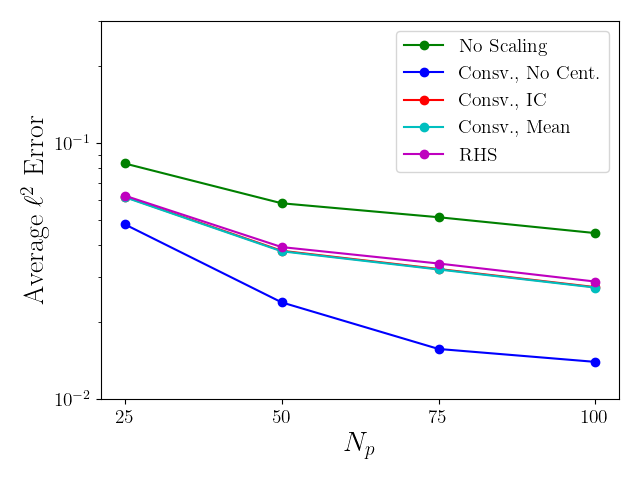
\includegraphics[width=0.99\linewidth]{Chapters/BestPractices/Images/errVsModes_norm_l2_Average_errorRaw.png}
		\subcaption{$\ell^2$-norm.}
	\end{minipage}
	\begin{minipage}{0.49\linewidth}
		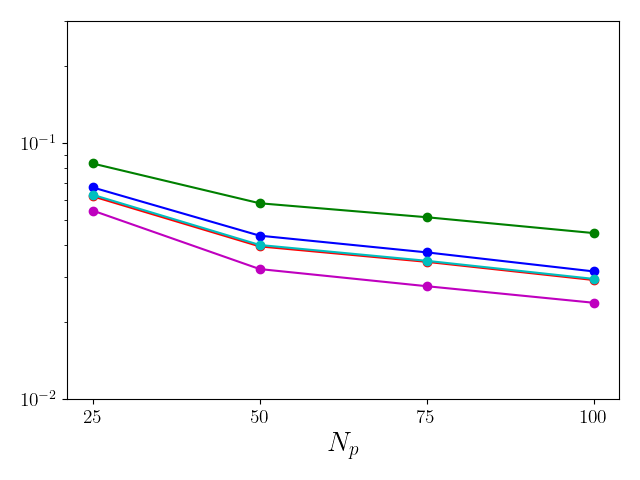
\includegraphics[width=0.99\linewidth]{Chapters/BestPractices/Images/errVsModes_norm_minmax_Average_errorRaw.png}
		\subcaption{Min-max.}
	\end{minipage}
	\caption{CVRC unsampled MP-LSVT PROM time-average error, $\numPrimModes = 25$, various residual scalings.}
\end{figure}

\begin{figure}
	\begin{minipage}{0.49\linewidth}
		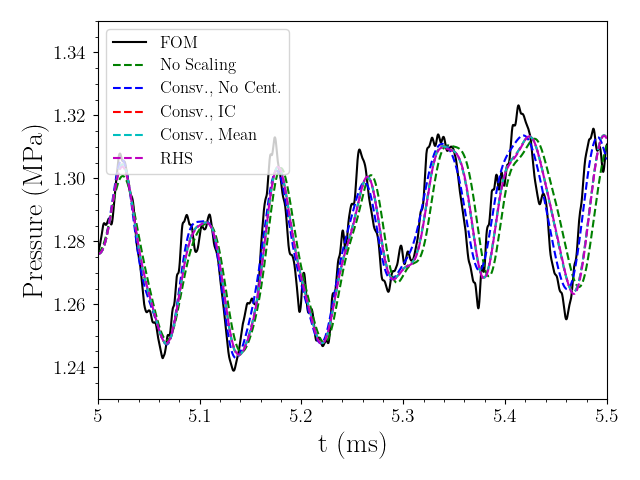
\includegraphics[width=0.99\linewidth]{Chapters/BestPractices/Images/pressure_probe_scale_l2.png}
		\subcaption{$\ell^2$-norm.}
	\end{minipage}
	\begin{minipage}{0.49\linewidth}
		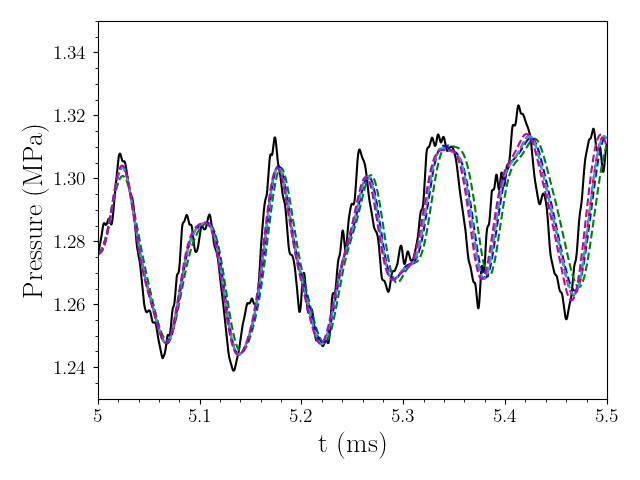
\includegraphics[width=0.99\linewidth]{Chapters/BestPractices/Images/pressure_probe_scale_minmax.png}
		\subcaption{Min-max.}
	\end{minipage}
	\caption{CVRC unsampled MP-LSVT PROM pressure probes, $\numPrimModes = 25$, various residual scalings.}
\end{figure}